\section{Métodos de avaliação}

A avaliação das proteínas geradas pelo agente é realizada em três etapas: 
análise estrutural, interação molecular por \textit{Docking} e imunogenicidade. 
Cada etapa é essencial para verificar se as proteínas geradas possuem características estruturais, 
funcionais e imunológicas adequadas para substituir o FIX no tratamento da hemofilia B.  

\subsection{Análise Estrutural}

A primeira etapa consiste em medir a similaridade estrutural entre cada proteína gerada
e o FIX por meio do \textit{TMScore}. 
Para isso, foi implementado um algoritmo que recebe como entrada o conjunto de sequências geradas $S_{gen}$,
a estrutura alvo $E_{FIX}$ e o modelo de predição estrutural $ESMFold$. 
Para cada sequência gerada, é feito a predição da estrutura tridimensional $E_S$ e o cálculo do \textit{TMScore} em
relação à estrutura alvo $E_{FIX}$.

\begin{algorithm}
  \caption{Avaliação Estrutural via TMScore}
  \label{alg:evaluation_tmscore}
  \begin{algorithmic}[1]
  \Require Conjunto de sequências geradas $S_{gen}$, 
  \State         estrutura alvo $E_{FIX}$,
  \State         modelo de predição estrutural $ESMFold$
  \Ensure Lista de TMScore para cada sequência gerada

  \State $TMScore\_list \gets []$
  \For{$S$ em $S_{gen}$}
      \State $E_S \gets ESMFold(S)$
      \State $TM_S \gets TMScore(E_{FIX}, E_S)$
      \State Adiciona $TM_S$ a $TMScore\_list$
  \EndFor
  \State \Return $TMScore\_list$
  \end{algorithmic}
\end{algorithm}

\subsection{Avaliação de Interação com o Fator VIII (Docking Molecular)}

Além da similaridade estrutural, é fundamental avaliar a capacidade das proteínas geradas 
de interagir corretamente com o Fator VIII (FVIII), replicando a função do FIX nativo. 
Para isso, realizamos análises de \textit{docking molecular} entre cada estrutura gerada e o FVIII,
utilizando métricas como \textit{Contact Molecular Surface} (CMS), \textit{Interface Buried SASA} (IBSASA), 
\textit{Delta Gibbs Free Energy of Binding} (DDG) e \textit{Surface Area Potential Score} (SAP Score) \ref{subsection:Docking}.

Antes da realização do \textit{docking}, é necessário alinhar estruturalmente a proteína gerada com o FVIII
para garantir que a proteína mutante ocupe a mesma posição relativa do FIX no complexo original. 
Isso é feito utilizando \textit{ChimeraX} (\cite{ChimeraX}) por meio do comando \texttt{matchmaker}, 
que alinha a estrutura gerada ao FIX presente no complexo tenase. 
O procedimento segue os seguintes passos: (i) carregamento do PDB do complexo tenase, 
(ii) carregamento do PDB da estrutura gerada, (iii) alinhamento da estrutura gerada sobrepondo-a ao FIX do complexo tenase 
e (iv) remoção do FIX original, mantendo apenas a estrutura gerada alinhada ao FVIII.
Esta implementação\footnote{Disponível em: \url{https://github.com/ArthurPimenta0306/Hallucination/blob/main/hpd/src/docking/ChimeraX_run_script.py}} está disponível
no repositório do projeto.

\begin{algorithm}
  \caption{Alinhamento Estrutural com ChimeraX}
  \label{alg:alignment_chimerax}
  \begin{algorithmic}[1]
  \Require Arquivo PDB do complexo tenase, arquivo PDB da estrutura gerada
  \Ensure Estrutura gerada alinhada ao FVIII

  \State Carregar PDB do complexo tenase
  \State Carregar PDB da estrutura gerada
  \State Alinhar a estrutura gerada ao FIX usando \textit{matchmaker}
  \State Remover o FIX do complexo
  \State \Return Estrutura gerada alinhada ao FVIII
  \end{algorithmic}
\end{algorithm}


\begin{figure}[H]
  \centering
  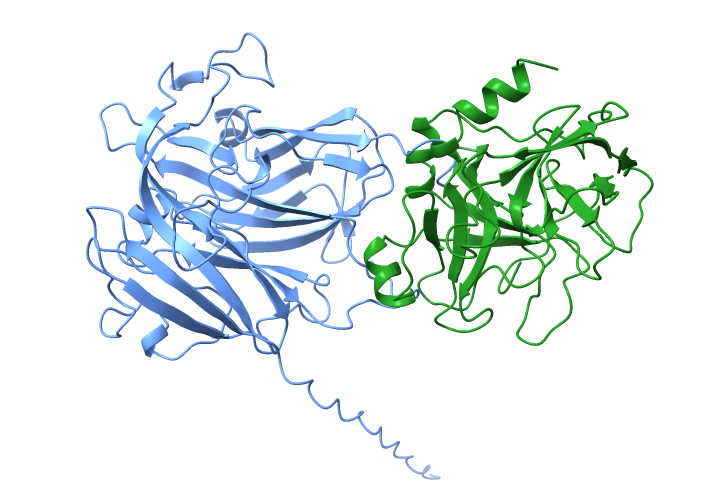
\includegraphics[width=.6\textwidth]{figuras/complexocomid63.png}
  \caption{Proteína gerada 63 (verde) alinhada com o FVIII (azul)}
\end{figure}

Após o alinhamento estrutural utilizando \textit{ChimeraX}, realizamos o \textit{docking molecular} 
por meio do protocolo \textit{Rosetta Docking}, 
que permite prever a orientação e estabilidade do complexo proteína-proteína gerado.
O \textit{Rosetta Docking} consiste em um procedimento iterativo que busca a conformação de menor energia livre do complexo.
O protocolo inicia com a geração de múltiplas poses, onde a proteína mutante é rotacionada e transladada em relação ao FVIII.
Em seguida, as conformações passam por um refinamento energético que inclui otimização da 
orientação relativa (\textit{rigid-body minimization}) e ajuste das cadeias laterais na interface 
(\textit{side-chain minimization}). 
O protocolo utiliza a função de energia do \textit{Rosetta} para estimar a estabilidade do complexo,
considerando fatores como interações de \textit{Van der Waals}, 
ligações de hidrogênio, energia eletrostática e solubilidade.
Baseado na função de energia e da posição relativa dos átomos no complexo, 
é calculada as métricas \textit{CMS}, \textit{IBSASA}, 
\textit{DDG} e \textit{SAP Score}.
O comando para execução do docking, 
bem como sua parametrização 
estão disponíveis\footnote{Disponível em: \url{https://github.com/ArthurPimenta0306/Hallucination/blob/main/hpd/src/docking/docking_protein_pipeline.sh} e \url{https://github.com/ArthurPimenta0306/Hallucination/blob/main/hpd/src/docking/main.py}}
e ilustrados a seguir.

\textbf{Comando para execução - \textit{Rosetta Docking}}
\begin{lstlisting}[language=bash, breaklines=true, frame=single, backgroundcolor=\color{lightgray}]
  ../rosetta.source.release-371/main/source/bin/docking_protocol.default.macosclangrelease -ignore_unrecognized_res @flag_file -out:prefix process_1_
\end{lstlisting}

\textbf{Parametrização - \textit{Rosetta Docking}}
\begin{enumerate}
    \item \textbf{ignore\_unrecognized\_res}: Atributo utilizado para ignorar resíduos não reconhecidos pelo \textit{Rosetta}.
    \item \textbf{flag\_file}: Arquivo .flag contendo os parâmetros de execução do \textit{Rosetta Docking}.
    \item \textbf{out:prefix}: Prefixo para os arquivos de saída gerados pelo \textit{Rosetta Docking}.
\end{enumerate}

\textbf{Parametrização - Arquivo .flag utilizado como \textit{input} do \textit{Rosetta Docking}}
\begin{enumerate}
    \item \textbf{in:file:s}: Especifica o caminho para o arquivo PDB do complexo de entrada (FVIII junto de uma proteína gerada), que será utilizada no processo de docking. Ex: \texttt{complex\_step\_1.pdb}
    \item \textbf{nstruct}: \texttt{1000}. Define o número de modelos (poses de encaixe entre as duas proteínas) a serem gerados no processo de \textit{docking}.
    \item \textbf{partners}: \texttt{A\_H}. Especifica quais cadeias da estrutura PDB interagem no \textit{docking}. 
    \item \textbf{dock\_pert}: \texttt{3 8}. Aplica uma perturbação inicial na orientação da proteína antes do docking. O primeiro valor (\texttt{3}) representa um deslocamento translacional em Ångströms, enquanto o segundo (\texttt{8}) define uma rotação em graus.
    \item \textbf{out:path:all}: Define o diretório onde todos os arquivos de saída do docking serão armazenados. Ex: \texttt{output\_files/} 
\end{enumerate}

A partir dos resultados do docking, implementamos
o processo que calcula as métricas responsáveis por quantificar 
a qualidade da interação entre as proteínas geradas e o FVIII utilizando o \textit{PyRosetta}\footnote{Disponível em: \url{https://github.com/ArthurPimenta0306/Hallucination/blob/main/hpd/src/docking/get_interface_metrics_small.py}}. 

\subsection{Avaliação da Imunogenicidade das Proteínas Geradas}

O objetivo desta etapa é identificar possíveis epítopos imunogênicos presentes nas sequências geradas, 
os quais poderiam desencadear respostas imunes indesejadas nos pacientes.
Para realizar esta análise, foi utilizado o \textit{NetMHCIIpan} versão 4.1 (\cite{Jensen2018NetMHCIIpan}), 
um dos algoritmos mais avançados para predição de ligação de peptídeos a moléculas 
do Complexo Principal de Histocompatibilidade de classe II (MHC II). 
O \textit{NetMHCIIpan} emprega técnicas de aprendizado de máquina para prever a afinidade de ligação de peptídeos 
derivados das proteínas analisadas às diferentes variantes alélicas de MHC II. 

O procedimento de execução do \textit{NetMHCIIpan} foi organizado em um \textit{script bash} 
que automatiza a análise de todas as sequências de proteínas geradas pelo modelo de otimização. 
Primeiramente, foi criado um arquivo denominado \texttt{selected\_alleles.txt}, 
o qual contém a lista dos alelos de MHC II humanos escolhidos para a análise. 
Estes alelos foram selecionados com o intuito de representar a diversidade populacional e garantir uma avaliação 
abrangente da imunogenicidade das variantes propostas.
Foram utilizados 46 alelos de MHC II frequentes na população humana, 
pertencentes aos grupos DP, DQ, DRB1 DRB3, DRB4 e DRB5.
Para cada alelo,
O \textit{script} itera sobre cada alelo presente no arquivo \texttt{selected\_alleles.txt}, 
invocando o \texttt{NetMHCIIpan} para todas as proteínas geradas.

\begin{lstlisting}[language=bash, breaklines=true, frame=single, backgroundcolor=\color{lightgray}]
  cores=2  
  while read p; do
      ls *.fasta | parallel -j $cores -k \
      "../netMHCIIpan-4.1/netMHCIIpan -a $p -f {} \
      -length 15,16,17,18,19,20 -BA -context > {}-$p-output.txt"
  done < selected_alleles.txt
\end{lstlisting}

\textbf{Parametrização - Análise Imunológica com \textit{NetMHCIIpan}}
\begin{enumerate}
    \item \textbf{cores}: 2. Número de núcleos de processamento utilizados para paralelização.
    \item \textbf{selected\_alleles.txt}: Arquivo contendo a lista dos alelos de MHC II humanos que serão utilizados na predição. Foram utilizados 46 alelos de MHC II frequentes na população humana, pertencentes aos grupos DP, DQ, DRB1 DRB3, DRB4 e DRB5.
    \item \textbf{length}: 15,16,17,18,19,20. Define os comprimentos dos peptídeos que serão extraídos da sequência e avaliados quanto à afinidade de ligação. Esses comprimentos são típicos de epítopos apresentados por MHC II.
    \item \textbf{BA}: Ativa o modo de predição baseado na afinidade de ligação (Binding Affinity).
    \item \textbf{context}: Habilita a consideração de regiões adjacentes aos peptídeos, o que aumenta a precisão da predição.
\end{enumerate}

Os arquivos gerados contêm a sequência do peptídeo analisado e
o valor de afinidade de ligação (IC50 em nM).
A partir desses resultados, foi realizada uma análise comparativa entre os 
peptídeos derivados das proteínas otimizadas e do FIX nativo.
Considerou-se como potenciais epítopos imunogênicos fortes aqueles peptídeos com valores de IC50 inferiores a 500 nM,
conforme recomendado por \cite{Jensen2018NetMHCIIpan}.
O número total de epítopos fortes, o \textit{Binding Affinity} 
e a frequência com que os alelos ocorrem na natureza são as métricas utilizadas
para avaliar e comparar a imunogenicidade das proteínas geradas com a proteína nativa \ref{section:imuno_resultados}. 

























